% Generate boilerplate to create a document with a title page, name, date with a report style
% Usage: \report{Title}{Name}{Date}

\documentclass{report}

\usepackage{graphicx}  % For including images
\usepackage{amsmath}   % For mathematical symbols and environments
\usepackage{hyperref}  % For hyperlinks
\usepackage{wrapfig}  % For wrapping text around figures

% Command to create the title page
\newcommand{\report}[3]{
    \title{#1}
    \author{#2}
    \date{#3}
    \maketitle
}

\begin{document}

% Create the title page
\report{Lyapunov Orbits}{Your Name}{\today}


\newpage

\section{Lyapunov Orbits}
\subsection{Dynamical model}
The dynamical model employed in this study is the planar circular restricted three-body problem (PCR3BP).
In this framework, the equation of motion are written in a non-dimensional form as follows:
\begin{equation}
    % [x_dd,y_dd] = 2[y_d,-x_d] + [U_x,U_y]
    \begin{bmatrix}
        \ddot{x} \\
        \ddot{y}
    \end{bmatrix}
    = 2
    \begin{bmatrix}
        \dot{y} \\
        -\dot{x}
    \end{bmatrix}
    +
    \begin{bmatrix}
        U_x \\
        U_y
    \end{bmatrix}
\end{equation}
where $x$ and $y$ are the non-dimensional position coordinates of the spacecraft.\\
U is the gravitational potential of the system, which is given by:
\begin{equation}
    U(x,y) = \frac{x^2 + y^2}{2} + \frac{1-\mu}{r_1} + \frac{\mu}{r_2}
\end{equation}
where $\mu$ is the mass ratio of the two primary bodies, and $r_1$ and $r_2$ are the distances from the spacecraft to the primary bodies.\\
The model is rewritten in the form $\dot{\boldsymbol{x}} = f(\boldsymbol{x})$ with:
\begin{equation}
    \boldsymbol{x} = 
    \begin{bmatrix}
        x \\
        y \\
        u \\
        v
    \end{bmatrix}  \quad \quad \quad \text{and} \quad \quad \quad 
    \begin{bmatrix}
        \dot{x} \\
        \dot{y} \\
        \dot{u} \\
        \dot{v}
    \end{bmatrix}
    =
    \begin{bmatrix}
        u \\
        v \\
        2v + U_x \\
        -2u + U_y
    \end{bmatrix}
\end{equation}
\subsection{Lagrangian points}

The Lagrangian points are equilibrium points in the phase space of the PCR3BP. 
The five Lagrangian points are denoted by $L_1$, $L_2$, $L_3$, $L_4$, and $L_5$. 
\begin{wrapfigure}{r}{0.5\textwidth}
    \centering
    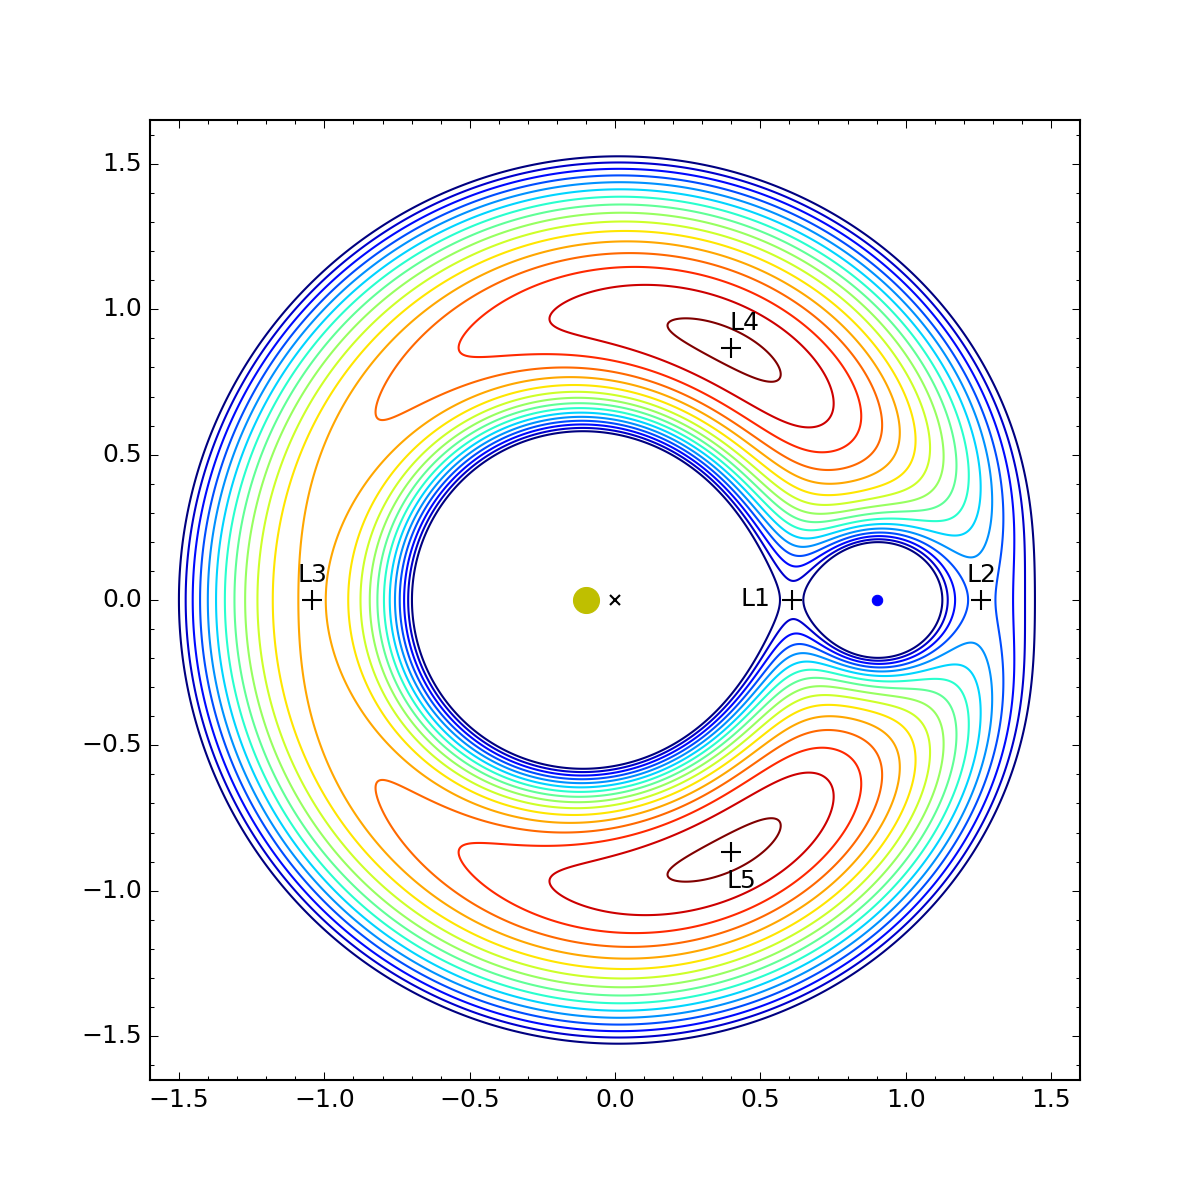
\includegraphics[width=0.5\textwidth]{images/Contour lines for Lagrange points.png}
    \caption{Lagrange points in the PCR3BP}
    \label{fig:lagrange_points}
\end{wrapfigure}
The first three points are collinear with the two primary bodies, while the last two are the 
third vertex of the equilateral triangle formed by the two primary bodies.\\\\\\
For Lyapunov orbits, we are interested in the $L_1$ and $L_2$ points. The phase space around
these points is of the type saddle-center in the planar case, with two real eigenvalues (one positive unstable
and one negative stable) and two complex conjugate eigenvalues.\\
The choosen binary system is the Earth-Moon system, but the results can be generalized
as long as the mass parameter $\mu$ is such that collinear points are unstable.

\subsection{Linearized motion around collinear equilibrium points}
With $\boldsymbol{x_L}$ the state of the generic collinear equilibrium point, the generic state
can be linearized around $\boldsymbol{x_L}$ as $\boldsymbol{x} = \boldsymbol{x_L} + \delta\boldsymbol{x}$

\chapter{Methodology}
% Your methodology content here

\chapter{Results}
% Your results content here

\chapter{Conclusion}
% Your conclusion content here

\end{document}